% \documentclass[CEJM,DVI]{cej} % use DVI command to enable LaTeX driver
\documentclass[CEJM,PDF]{cej} % use PDF command to enable PDFLaTeX driver
\usepackage{layout}


\def\lorem{Lorem ipsum dolor sit amet, consectetur adipisicing elit, sed do eiusmod tempor incididunt ut labore et dolore magna aliqua. Ut enim ad minim veniam, quis nostrud exercitation ullamco laboris nisi ut aliquip ex ea commodo consequat. Duis aute irure dolor in reprehenderit in voluptate velit esse cillum dolore eu fugiat nulla pariatur. Excepteur sint occaecat cupidatat non proident, sunt in culpa qui officia deserunt mollit anim id est laborum.}

\def\LOREM{\lorem \\ \lorem}



\title{Title of the article}

\articletype{Article category} % Research Article, Review Article, Communication, Erratum




\author{First~Author\inst{1}\email{email@first.author.com},
        Second~Author\inst{2}\email{email@second.author.com}
       }

\shortauthor{F. Author, S. Author}

\institute{\inst{1}
           Department of Mathematics, University Full Name, Street, Postal code, City, Country
           \inst{2}
           Institute of Mathematics, Research Institution, Street, Postal code, City, Country
          }

\abstract{An abstract should accompany every article. It should be a brief summary of significant results of the paper. An abstract should give concise information about the content of the core idea of your paper. It should be informative and not only present the general scope of the paper but also indicate the main results and conclusions.\\
The abstract should not exceed 200 words. It should not contain literature citations, allusions to the tables, tables, figures or illustrations. All nonstandard symbols and abbreviations should be defined. In combination with the title and keywords, an abstract is an indicator of the content of the paper.
}

\keywords{Keyword 1 \*\ Keyword 2 \*\ Keyword 3}

\msc{XXXXX, YYYYY}

\begin{document}
\maketitle
%\baselinestretch{2}
\section{Introduction }

Some introductory text. Some introductory text. Some introductory text. Some introductory text. Some introductory text. Some introductory text. Some introductory text. Some introductory text. Some introductory text. Some introductory text. Some introductory text. Some introductory text. Some introductory text. Some introductory text. Some introductory text. Some introductory text. Some introductory text. Some introductory text. Some introductory text. Some introductory text. Some introductory text. Some introductory text. Some introductory text. Some introductory text. Some introductory text. Some introductory text.




\section{Sample section}


Sample theorem with citation:

\begin{theorem}[Pythagoras \cite{euclid00}]\label{Pythagoras-famous}
Let $a,b,c$ denote the sides of a triangle. If the angle between $a,b$ equals $90^\circ$ then
$$|a|^2 + |b|^2 = |c|^2.$$
Moreover, regardless of the assumption on the angle, it holds that $|a|+|b|\ge |c|$.
\end{theorem}

See References for the bibliography style in CEJM.
Below is a proposition with a proof.

\begin{proposition}\label{Standard-stuff}
The only possible real solutions of the quadratic equation $ax^2+bx+c=0$ are
$$x_1 = \frac{-b-\sqrt{\Delta}}{2a} \qquad\text{and}\qquad x_2 = \frac{-b+\sqrt{\Delta}}{2a},$$
where $\Delta = b^2-4ac$.
\end{proposition}

\begin{proof}
Observe that
\begin{equation}
(x-x_1)\,(x-x_2) = -{\frac{\Delta}{4\,a^2}}+x^2+{\frac{b\,x}{a}}+{\frac{b^2}{4\,a^2}}
\label{eq-somelabel}
\end{equation}
Taking into account that $\Delta = b^2-4ac$, equation (\ref{eq-somelabel}) leads to
\begin{equation}
(x-x_1)\,(x-x_2) = \frac{c}{a}+x^2 + \frac{b\,x}{a}
\label{eq-anotherlabel}
\end{equation}
Finally, (\ref{eq-anotherlabel}) shows that $a\,(x-x_1)\,(x-x_2)$ equals the original equation.
A polynomial of degree two cannot have more than two roots, therefore $x_1,x_2$ are the only possible solutions of our equation.
\end{proof}

\begin{corollary}
If $b^2<4ac$ then the quadratic equation $ax^2+bx+c=0$ has no real solutions.
\end{corollary}

\subsection{Subsections and sample formulas}

This is a subsection.

Typical aligned list of formulas with labels, displayed by using the \verb align environment.
\begin{align}
\label{eq:first}
\left(b+a\right)\,\left(2\,b-3\,a\right) &= 2\,b^2-a\,b-3\,a^2\\
\label{eq:second}
123+321 &= 444
\end{align}
The same list without labels.
\begin{align*}
\left(b+a\right)\,\left(2\,b-3\,a\right) &= 2\,b^2-a\,b-3\,a^2\\
123+321&=444
\end{align*}
Now the same list with custom tags.
\begin{align*}
\label{eq:smallstars}
\left(b+a\right)\,\left(2\,b-3\,a\right) &= 2\,b^2-a\,b-3\,a^2
\tag*{$(**)$}\\ %<-- \tag* does not add parentheses
\label{eq:doubledagger}
123+321&=444
\tag{$\ddagger$} %<-- \tag adds parentheses
\end{align*}
Another example of aligned formulas
\begin{align*}
  1+1&=2    &    1+2&=3    &    1+3&=4   \\
\intertext{with some text inserted between,}
 10+1&=11   &   10+2&=12   &   10+3&=13  \\
100+1&=101  &  100+2&=102  &  100+3&=103
\end{align*}
by using the \verb \intertext command.





\subsubsection{Polynomials of degree three}

This is a ``subsubsection".

Below is a complicated formula, which must be divided into several lines using, for instance, the
\verb align* \ environment:
\begin{align*}
x_1 &= \left(-{{\sqrt{3}\,i}\over{2}}-{{1}\over{2}}\right)\, \left({{3^ {- {{3}\over{2}} }\,\sqrt{12\,a^4-12\,a^3+188\,a^2-432\,a +247}}\over{2}}-{{2\,a^3+72\,a-81}\over{54}}\right)^{{{1}\over{3}}}\\
&+ {{\left({{\sqrt{3}\,i}\over{2}}-{{1}\over{2}}\right)\,\left(a^2-3 \right)}\over{9\,\left({{3^ {- {{3}\over{2}} }\,\sqrt{12\,a^4-12\,a^3 +188\,a^2-432\,a+247}}\over{2}}-{{2\,a^3+72\,a-81}\over{54}}\right) ^{{{1}\over{3}}}}}-{{a}\over{3}},\\
x_2 &= \left({{\sqrt{3}\,i}\over{2}}- {{1}\over{2}}\right)\,\left({{3^ {- {{3}\over{2}} }\,\sqrt{12\,a^4-12 \,a^3+188\,a^2-432\,a+247}}\over{2}}-{{2\,a^3+72\,a-81}\over{54}} \right)^{{{1}\over{3}}}\\
&+{{\left(-{{\sqrt{3}\,i}\over{2}}-{{1}\over{2 }}\right)\,\left(a^2-3\right)}\over{9\,\left({{3^ {- {{3}\over{2}} } \,\sqrt{12\,a^4-12\,a^3+188\,a^2-432\,a+247}}\over{2}}-{{2\,a^3+72\, a-81}\over{54}}\right)^{{{1}\over{3}}}}}-{{a}\over{3}},\\
x_3 &= \left({{3 ^ {- {{3}\over{2}} }\,\sqrt{12\,a^4-12\,a^3+188\,a^2-432\,a+247} }\over{2}}-{{2\,a^3+72\,a-81}\over{54}}\right)^{{{1}\over{3}}}\\
&+{{a^2 -3}\over{9\,\left({{3^ {- {{3}\over{2}} }\,\sqrt{12\,a^4-12\,a^3+188 \,a^2-432\,a+247}}\over{2}}-{{2\,a^3+72\,a-81}\over{54}}\right)^{{{1 }\over{3}}}}}-{{a}\over{3}}
\end{align*}

\begin{theorem}\label{th_poly3}
The numbers $x_1,x_2,x_3$ defined above are the only complex solutions of the equation
$$x^3+a\,x^2+x+3\,\left(a-1\right)=0.$$
\end{theorem}

\begin{proof}
Easy calculations, using \href{http://maxima.sourceforge.net/}{Maxima} or some other free computer algebra system.
\end{proof}


\paragraph{Other polynomials}

This is a paragraph with title.

One should admit that there is no general formula for the solutions of general polynomial equations and therefore sometimes we must use numerical methods.

\begin{example}\label{examp-123}
Consider the polynomial $v(t)=t^3+t+1$ of degree three. It turns out that its only real root is
$$t=\left({{3^ {- {{3 }\over{2}} }\,\sqrt{31}}\over{2}}-{{1}\over{2}}\right)^{{{1}\over{3 }}}-{{1}\over{3\,\left({{3^ {- {{3}\over{2}} }\,\sqrt{31}}\over{2}}- {{1}\over{2}}\right)^{{{1}\over{3}}}}}$$
There are also other two complex roots\footnote{Since the degree of $v$ is $3$, we know that there may be at most $3$ roots.}, which we ignore.
\end{example}


\begin{remark}\label{rem_CAS}
The proof of Theorem \ref{th_poly3} uses some advanced technology, including a computer algebra system. The same applies to Example \ref{examp-123}. On the other hand, Proposition \ref{Standard-stuff} is well known and its proof is rather elementary.
\end{remark}





\section{Tables and figures}

Table \ref{tab-01} shows how to show some data using the \verb table environment.

\begin{table}
\def~{\phantom0}
\catcode`\@=13
\def@{\phantom.}
\caption{Some caption text.\label{tab-01}}
\medskip
\begin{center}
\begin{tabular}{l|ccc}\hline
\multicolumn1l{\it Some title}\\\hline\hline
row 1, column 1         &   row 1, column 2  \\
row 2, column 1    &   row 2, column 2   \\
row 3, column 1    &   row 3, column 2   \\
\hline
\multicolumn1l{\it Another title} & Value 1 &   Value 2 &   Value 3 \\
\hline\hline
row 1                    & ~130 & 30 & 30 \\
row 2                    & 1025 & ~1 & 15 \\
row 3                   & ~100 & ~1 & 10 \\
row 4        & 2925 & ~1 & ~4 \\
row 5            & 2950 & ~1 & ~2 \\\hline
\end{tabular}
\end{center}
\end{table}

Figure \ref{fig_abc} shows how to use the \verb figure environment for displaying graphics, etc.

\begin{figure}
\caption{The graph of $y=x\,sin x$ in the interval [-50,50], created by wxMaxima 0.7.4. \label{fig_abc}}
%\vskip3cm
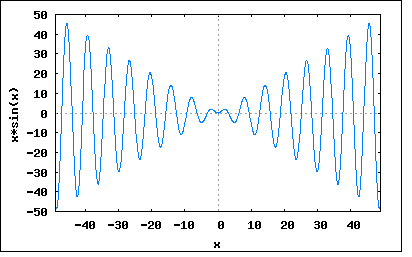
\includegraphics{xsinx-49.png}
\end{figure}


\section*{Acknowledgements}

The author(s) would like to thank some institutions for support and so on.


\begin{thebibliography}{9}

\bibitem{annis-etal} Anninis K., Crabi T.J., Sunday T.J., New methods for parallel computing, In: Lyonvenson S. (Ed.), Proceedings of Computer Science Conference (1-�10 Jul. 2007 Haifa Israel), University Press, 2007, 13�-179

\bibitem{p1} Author N., Coauthor M., Title of article, J. Some Math., 2007, 56, 243--256

\bibitem{katish} Katish A., The inconsistency of ZFC, preprint available at
http://arxiv.org/abs/1234.1234

\bibitem{kittel_etal} Kittel S.J., Maria G., Tuke M., Sepran D.J., Smith J., Tadeuszewicz K., et al., New class of measurable functions, J. Real Anal., 1997, 999, 234-�255

\bibitem{nowak1} Nowak P., New axioms for planar geometry, Eastern J. Math., 1999, 1, 324�-334, (in Polish)

\bibitem{nowak} Nowak P., Even better axioms for planar geometry, Eastern J. Math., (in press, in Polish), DOI: 33.1122/321

\bibitem{euclid00} Pythagoras S., On the squares of sides of certain triangles, J. Ancient Math., 2003, 4, 1--30, (in Greek)

\bibitem{sambrook} Sambrook J., Uncountable abelian groups, In: Sambrook J., Russell D.W. (Eds.), Contributions to Abelian groups, 3rd ed., Nauka, Moscow, 2001

\bibitem{sambrook-russell} Sambrook J., Russell D.W., Abelian groups, 3rd ed., Nauka, Moscow, 2001

\end{thebibliography}

\end{document}
